\documentclass[11pt,fleqn]{book}
\usepackage[top=3cm,bottom=3cm,left=3.2cm,right=3.2cm,headsep=10pt,letterpaper]{geometry}
						\usepackage{xcolor}
						\definecolor{ocre}{RGB}{52,177,201} 
						\usepackage{avant} 
						\usepackage{mathptmx}
						\usepackage{microtype}
						\usepackage[utf8]{inputenc}
						\usepackage[T1]{fontenc} 
						\usepackage[style=alphabetic,sorting=nyt,sortcites=true,autopunct=true,babel=hyphen,hyperref=true,abbreviate=false,backref=true,backend=biber]{biblatex}
						\defbibheading{bibempty}{}
						\input{structure} 
						\begin{document}
\begingroup
\thispagestyle{empty}
\AddToShipoutPicture*{\put(0,0){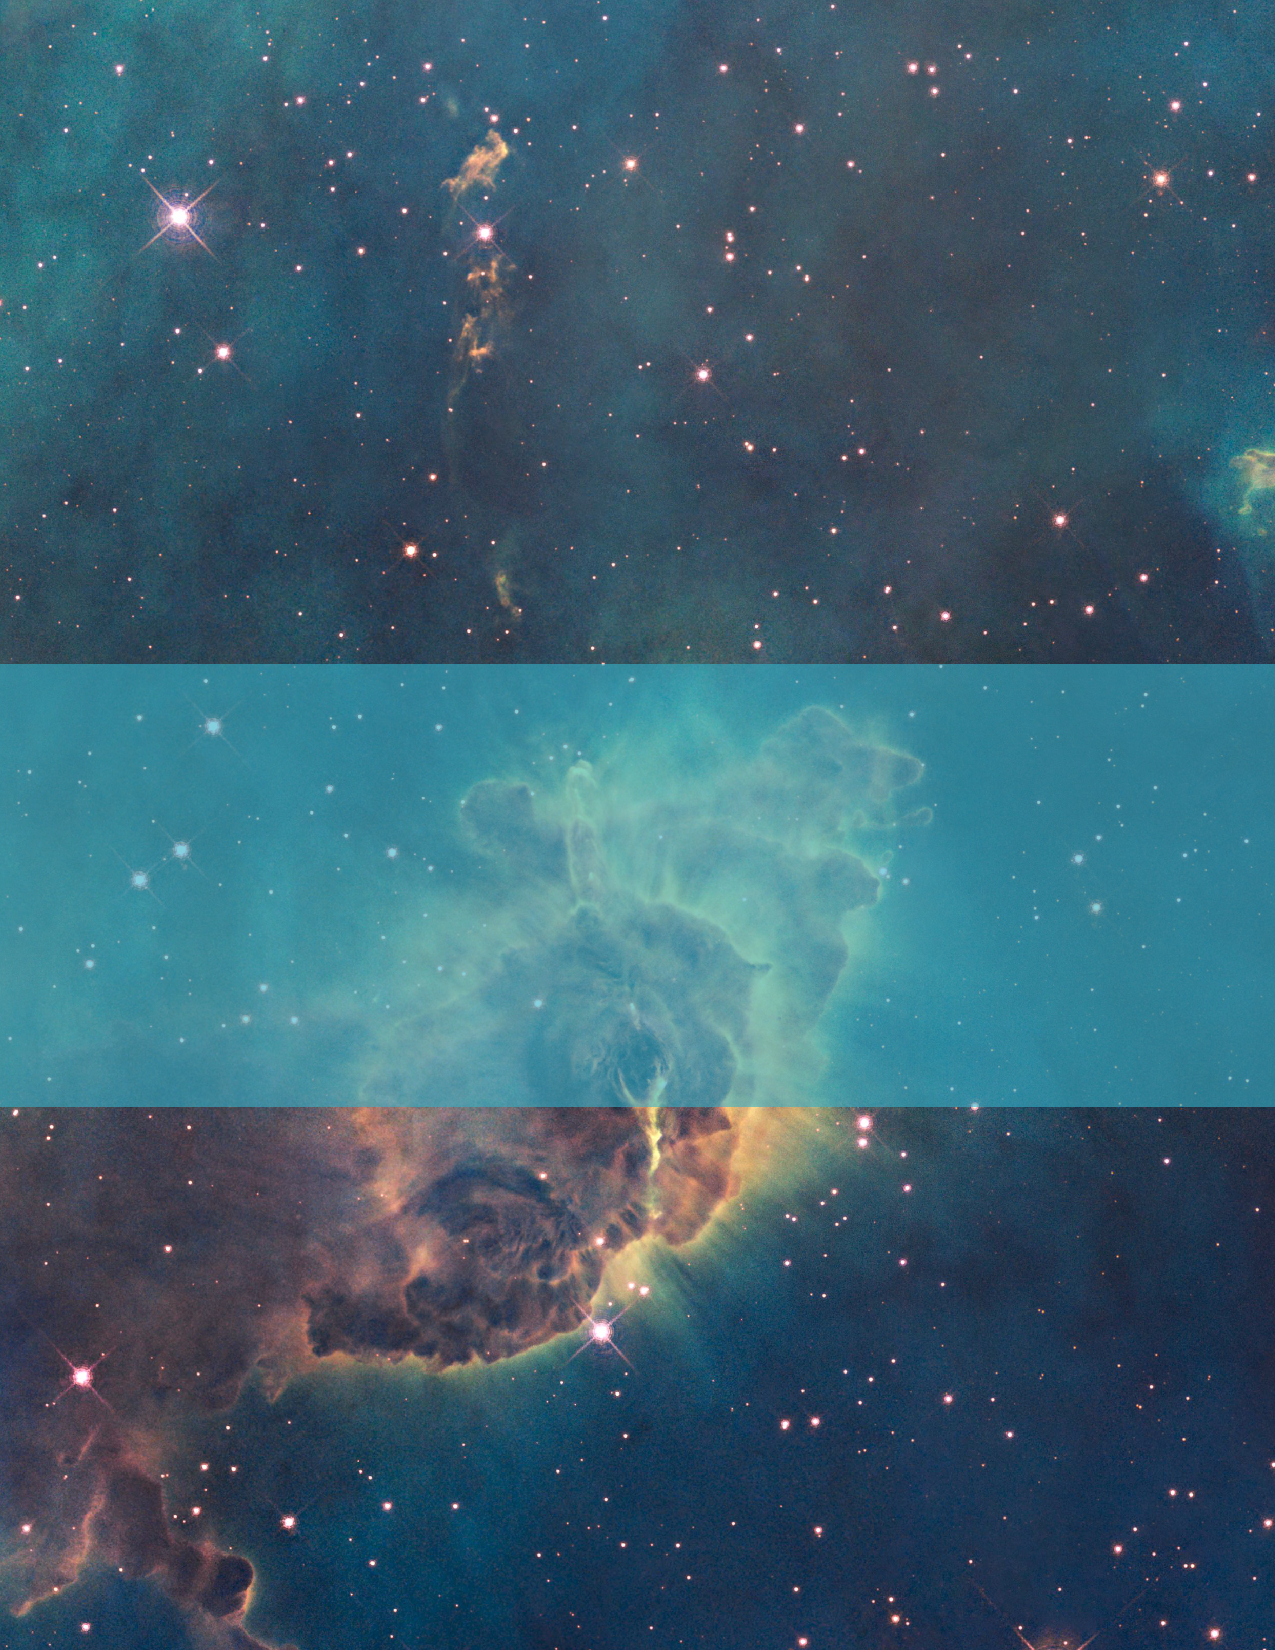
\includegraphics[scale=1.25]{esahubble}}} % Image background
\centering
\vspace*{5cm}
\par\normalfont\fontsize{35}{35}\sffamily\selectfont
\vspace*{2cm}
\textbf{Titre du document}\
~\\
{\Huge NOM PRENOM}\par % Author name
\endgroup
\chapterimage{head1.png} % Table of contents heading image
							\pagestyle{empty} % No headers
							\tableofcontents % Print the table of contents itself
							%\cleardoublepage % Forces the first chapter to start on an odd page so it's on the right
							\pagestyle{fancy} % Print headers again
\chapterimage{head1.png}
								\chapter{Partie 1}
\section{Sous partie 1}
Texte  ...
~\\
\includegraphics{./}
legende image
~\\
\begin{itemize}
\item choix  1
\item choix  2
\item choix  3
\end{itemize}
~\\
\begin{enumerate}
\item item  1
\item item  2
\item item  3 
\end{enumerate}
~\\
texte  en  \textit{gras*} ,  en  \textbf{italique*} et  en  \textbf{\textit{gras et italique}}
~\\
~\\
\begin{tabular}
{|l|l|}
\hline
colonne1 & colonne 2\\
\hline
valeur  1 & valeur  2\\
valeur  3 & valeur  4\\
\hline
\end{tabular}
~\\
~\\
\end{document}
